% --------------------------------------------------------------------------------

\begin{exercise}[Random walk of a robot]

A robot is placed at the origin (the point $(0, 0)$) on a two-dimension integer grid (see the figure below).
Denote the position of the robot by $(x, y)$.
The robot can either move right to $(x + 1, y)$ or move up to $(x, y + 1)$.

\begin{center}
    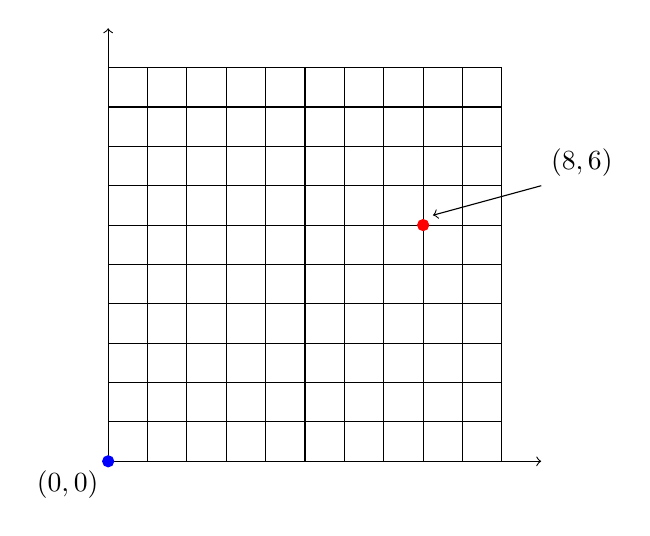
\begin{tikzpicture}[scale = 0.5]

        \draw [->] (0, 0) -- (0, 11);
        \draw [->] (0, 0) -- (11, 0);
        \draw (0, 0) grid (10, 10);

        \filldraw [color = blue] (0, 0) circle (4pt);
        \draw node [below left] {$(0, 0)$};

        \filldraw [color = red] (8, 6) circle (4pt);
        \draw [->] (11, 7) node [above right] {$(8, 6)$} -- (8.25, 6.25);

    \end{tikzpicture}
\end{center}

\begin{enumerate}[label = (\alph*)]

    \item Suppose each time the robot randomly moves right of up with equal chance.
    What is the probability that the robot will ever reach the point $(8, 6)$?

    \item Suppose another robot has a $\frac{2}{3}$ chance to move right and a $\frac{1}{3}$ chance to move up when $x + y$ is even, otherwise it has a $\frac{1}{4}$ chance to move right and a $\frac{3}{4}$ chance to move up.
    It stops whenever $|x - y| \geq 2$.
    Find the probability that $x - y = 2$ when it stops.

\end{enumerate}

\end{exercise}

% --------------------------------------------------------------------------------

\begin{solution}

\phantom{}

\begin{center}
    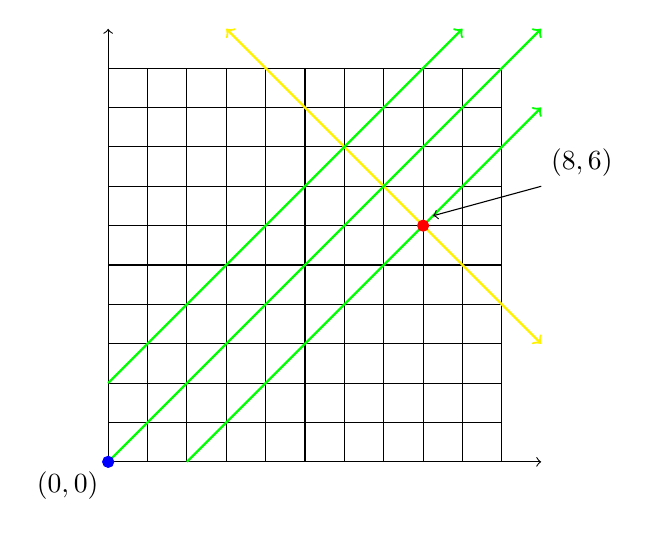
\begin{tikzpicture}[scale = 0.5]

        \draw [->] (0, 0) -- (0, 11);
        \draw [->] (0, 0) -- (11, 0);
        \draw (0, 0) grid (10, 10);

        \draw [<->, color = yellow, thick] (11, 3) -- (3, 11);

        \draw [->, color = green, thick] (0, 0) -- (11, 11);
        \draw [->, color = green, thick] (0, 2) -- (9, 11);
        \draw [->, color = green, thick] (2, 0) -- (11, 9);

        \filldraw [color = blue] (0, 0) circle (4pt);
        \draw node [below left] {$(0, 0)$};

        \filldraw [color = red] (8, 6) circle (4pt);
        \draw [->] (11, 7) node [above right] {$(8, 6)$} -- (8.25, 6.25);

    \end{tikzpicture}
\end{center}

\begin{enumerate}[label = (\alph*)]

    \item Each path that the robot moves along is equally likely.
    
    There are $\binom{a}{b}$ paths ($a = x + y$, $b \in \Bbraces{x, y}$) that lead from $(0, 0)$ to $(x, y)$.
    This can be observed by turning one of the figures above by $90 + 45$ degrees clockwise and modifying it to be a Pascal's triangle.
    The number of downwards paths that lead from the root of a Pascal's to one of its nodes with value $z$ is $z$.
    
    \begin{figure}[H]
        \centering
        \subfloat[\href{https://de.m.wikipedia.org/wiki/Datei:Pascal_triangle_small.svg}{wikipedia}]{
            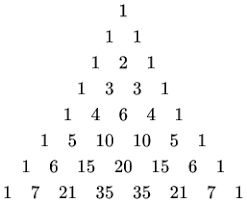
\includegraphics[width = 0.35 \textwidth]{pascals_triangle_wikipedia.png}
        }
        \hspace{1cm}
        \subfloat[\href{https://stackoverflow.com/questions/47614514/how-can-i-modify-my-program-to-print-out-pascals-triangle}{stackoverflow}]{
            
\includegraphics[width = 0.35 \textwidth]{pascals_triangle_stackoverflow.png}
        }
        \caption{Pascale's triangles}
    \end{figure}
    
    Let the robot move $8 + 6$ steps.
    It must land on the yellow diagonal $\Bbraces{(10, 4), \dots, (4, 10)}$.
    The position on that diagonal completely determines, whether the robot reaches $(8, 6)$ or not (since it can only move right and up).
    Consider the Binomial Theorem for $(1 + 1)^n$.
    
    \begin{align*}
        P(\text{robot passes through $(8, 6)$})
        & =
        P(\text{robot sits on $(8, 6)$} \mid \text{robot moved exactly $8 + 6$ steps}) \\
        & =
        \frac
        {
            \binom{14}{7 \pm 1}
        }{
            \sum_{n=0}^{14}
                \binom{14}{n}
        } \\
        & =
        \frac{\binom{14}{7 \pm 1}}{2^n} \\
        & \approx
        0.183288574219
    \end{align*}

    \item On the middle green diagonal $\Bbraces{(x, x)}_{x=0}^{10}$ every element $(x, x)$ has an even value $x + x$.

    $\Forall x = 0, \dots, 8:$

    \begin{align*}
        &
        P(\text{robot will move to $(x+1, x+1)$} \mid \text{robot sits at $(x, x)$}) \\
        & =
        P(\text{robot will move up and then right} \mid \text{robot sits at $(x, x)$}) \\
        & +
        P(\text{robot will move right and then up} \mid \text{robot sits at $(x, x)$}) \\
        & =
        \frac{1}{3} \frac{1}{4} + \frac{2}{3} \frac{3}{4} \\
        & =
        \frac{7}{12} =: p_0,
    \end{align*}

    \begin{align*}
        P(\text{robot will move to $(x+2, x)$} \mid \text{robot sits at $(x, x)$})
        =
        \frac{1}{3} \frac{3}{4}
        =
        \frac{3}{12} =: p_{-1},
    \end{align*}

    \begin{align*}
        P(\text{robot will move to $(x, x+2)$} \mid \text{robot sits at $(x, x)$})
        =
        \frac{2}{3} \frac{1}{4}
        =
        \frac{2}{12} =: p_1
    \end{align*}

    \begin{multline*}
        \pi_n
        :=
        P(\text{ending position $(x, y)$ fulfills $x - y = 2$} \mid x + y \leq 2 n) \\
        \xrightarrow{n \to \infty}
        P(\text{ending position $(x, y)$ fulfills $x - y = 2$}) =: \pi_\infty
    \end{multline*}

    \begin{align*}
        \pi_1 & = p_1 \\
        \pi_2 & = \pi_1 + p_0 p_1 = p_1 + p_0 p_1 = p_1 (1 + p_1) \\
        \pi_3 & = \pi_2 + p_0^2 p_1 = p_1 (1 + p_0) + p_0^2 p_1 = p_1 (1 + p_0 + p_0^2) \\
        & \vdots \\
        \pi_\infty & = p_1 \sum_{k=0}^\infty p_0^k = \frac{p_1}{1 - p_0} = \frac{2 / 12}{1 - 7 / 12} = \frac{2 / 12}{5 / 12} = \frac{2}{5} = 0.4
    \end{align*}

    \begin{comment}

        \begin{align*}
            &
            P(\text{ending position $(x, y)$ fulfills $|x - y| \neq 2$}) \\
            & =
            P
            \pbraces
            {
                \begin{array}{l}
                    \text{ending position is $(10, 10)$ and} \\
                    \text{robot only moves between diagonals $\Bbraces{(x+2, x)}_{x=0}^8$ and $\Bbraces{(x, x+2)}_{x=0}^8$}
                \end{array}
            } \\
            & =
            \underbrace
            {
                P(\text{robot will move to $(10, 10)$} \mid \text{robot sits at $(9, 9)$})
            }_1 \\
            & \quad
            P(\text{robot will move to $(9, 9)$} \mid \text{robot sits at $(8, 8)$}) \\
            & \quad
            \vdots \\
            & \quad
            P(\text{robot will move to $(1, 1)$} \mid \text{robot sits at $(0, 0)$}) \\
            & =
            \prod_{x=0}^8
                P(\text{robot will move to $(x+1, x+1)$} \mid \text{robot sits at $(x, x)$}) \\
            & =
            \pbraces{\frac{7}{12}}^9
        \end{align*}

        \begin{align*}
            P(\text{ending position $(x, y)$ fulfills $x - y = 2$})
            =
            P(\text{ending position $(x, y)$ fulfills $|x - y| = 2$}) / 2
            =
            \pbraces{1 - \pbraces{\frac{7}{12}}^9} / 2
            \approx
            0.496089600308
        \end{align*}

    \end{comment}

\end{enumerate}

\end{solution}

% --------------------------------------------------------------------------------
